\documentclass[border=10pt]{standalone}

\usepackage{tikz}
\usepackage{tikzsymbols}
\usetikzlibrary{calc,patterns,shapes.geometric}

\def\centerarc[#1](#2)(#3:#4:#5){\draw[#1] ($(#2)+({#5*cos(#3)},{#5*sin(#3)})$) arc (#3:#4:#5);}

\begin{document}
	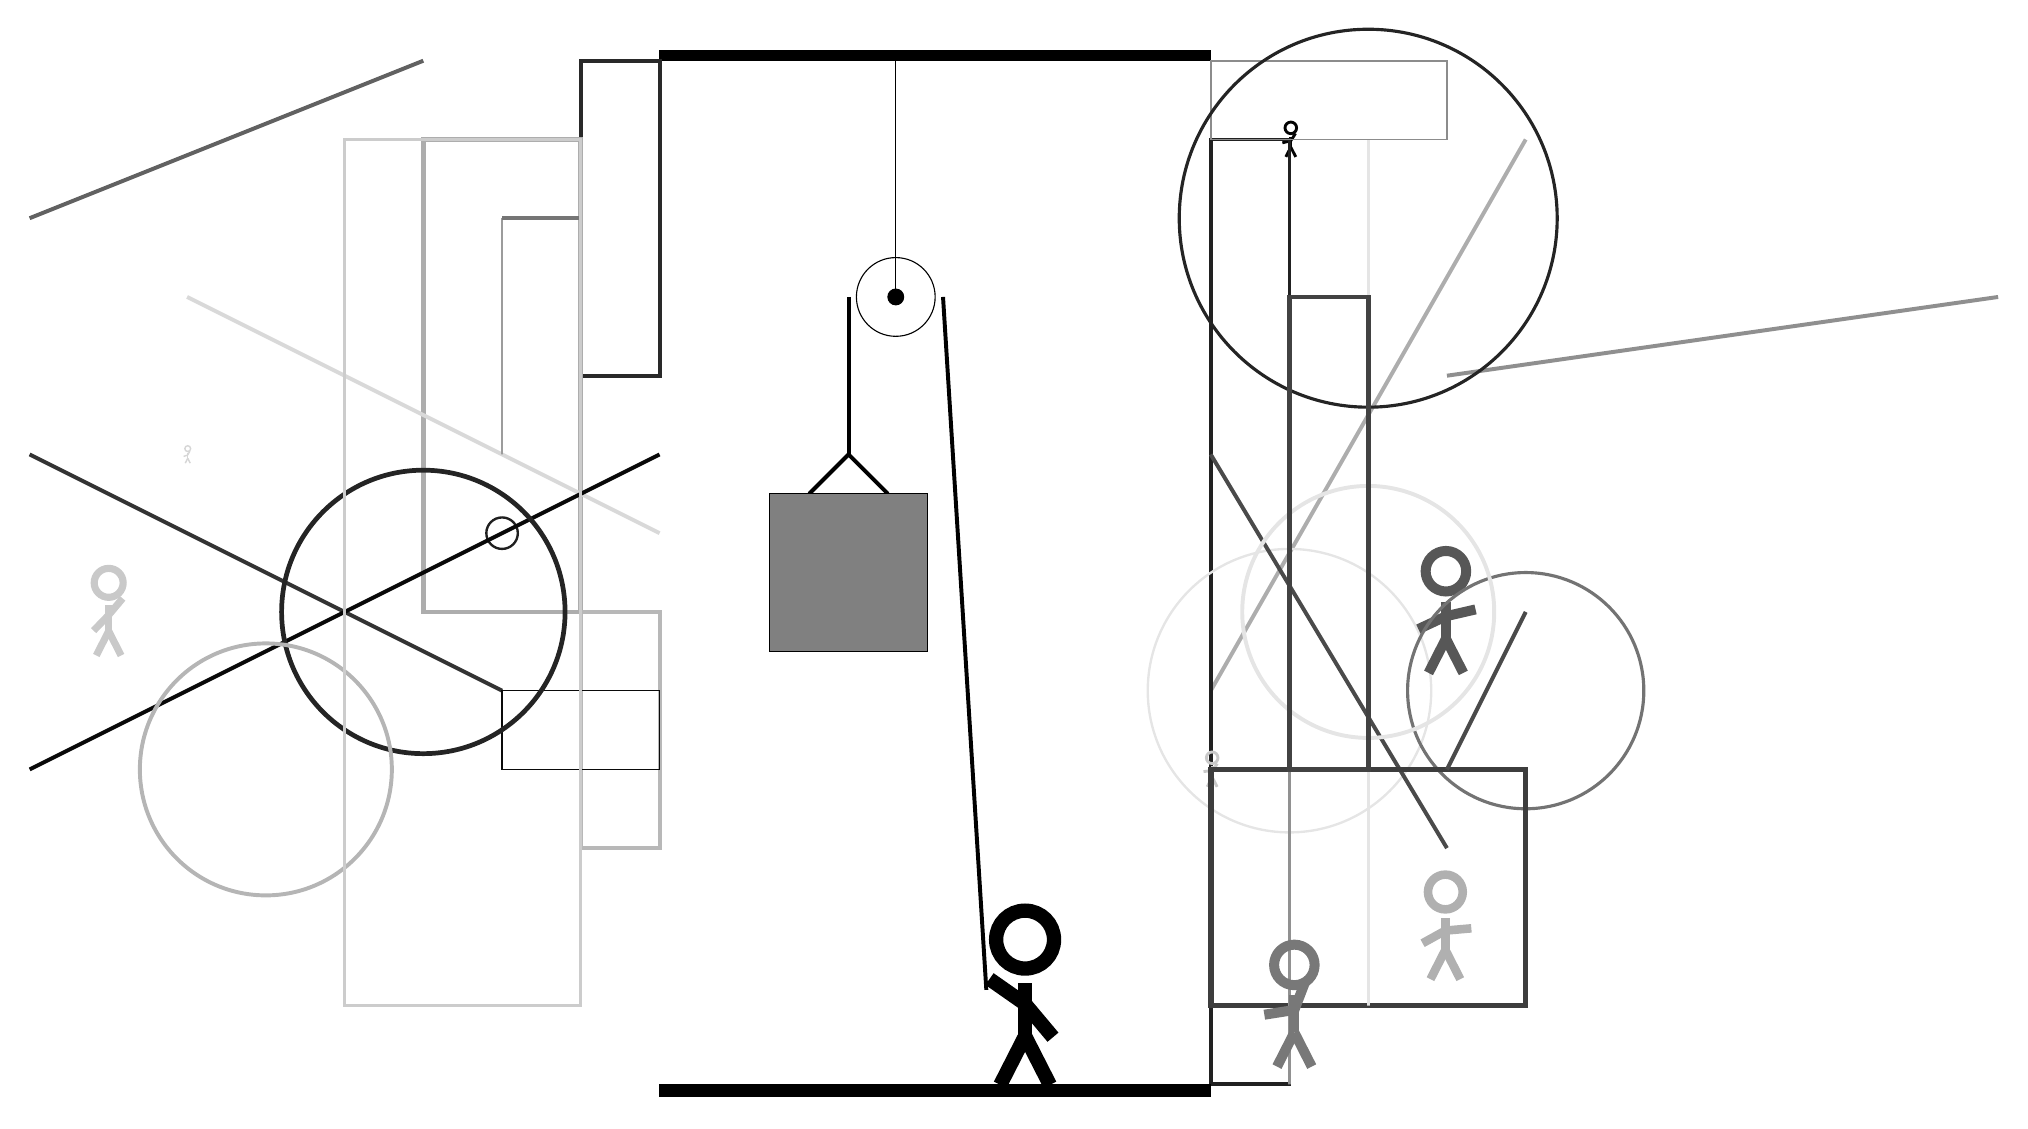
\begin{tikzpicture}
		%%%%% START %%%%%
		
		\draw[fill=black] (-2, 10) rectangle (5, 10.125);
		
		\draw (1, 7) circle (0.5);
		\draw[fill=black] (1, 7) circle (0.1);
		\draw (1, 10) -- (1, 7);
		
		\draw[line width=0.5mm] (-0.1, 4.5) -- (0.4, 5.0) -- (0.9, 4.5);
		\draw[fill=black!50] (-0.6, 4.5) rectangle (1.4, 2.5);
		
		\draw[line width=0.5mm] (0.4, 7) -- (0.4, 5.0);
		\centerarc[line width=0.5mm](1, 7)(0:180:0.6);
		\draw[line width=0.5mm](1.6, 7) -- (2.15, -1.8);
		
		\draw[line width=0.5mm, color=black!32](9, 9) -- (5, 2);
		
		\draw[line width=0.5mm, color=black!84] (-2, 6) rectangle (-3, 10);
		\node[line width=0.3mm, color=black!99] at (6, 9) {\Strichmaxerl[2][14][57]};
		\draw[line width=0.5mm, color=black!87] (6, 9) rectangle (5, -3);
		
		\draw[line width=0.5mm, color=black!62](-5, 10) -- (-10, 8);
		
		\draw[line width=0.5mm, color=black!80](-4, 2) -- (-10, 5);
		\node[line width=0.5mm, color=black!21] at (-9, 3) {\Strichmaxerl[5][46][50]};
		\draw [line width=0.3mm, color=black!10](6, 2) circle (1.8);
		\draw[line width=0.5mm, color=black!71](5, 5) -- (8, 0);
		
		\node[line width=0.7mm, color=black!21] at (5, 1) {\Strichmaxerl[2][6][53]};
		
		\node[line width=0.3mm, color=black!66] at (8, 3) {\Strichmaxerl[7][25][13]};
		\draw [line width=0.7mm, color=black!81](-7, 7) circle (0.0);
		\draw [line width=0.4mm, color=black!55](9, 2) circle (1.5);
		
		\draw[line width=0.6mm, color=black!32] (-3, 9) rectangle (-5, 3);
		\node[line width=0.2mm, color=black!31] at (8, -1) {\Strichmaxerl[6][29][5]};
		\draw[line width=0.5mm, color=black!15](-2, 4) -- (-8, 7);
		
		\draw [line width=0.3mm, color=black!88](-4, 4) circle (0.2);
		\draw[line width=0.5mm, color=black!97](-2, 5) -- (-10, 1);
		\draw[line width=0.7mm, color=black!76] (5, 1) rectangle (9, -2);
		
		\draw [line width=0.5mm, color=black!10](7, 3) circle (1.6);
		\draw[line width=0.4mm, color=black!10] (7, 9) rectangle (7, -2);
		
		\draw[line width=0.5mm, color=black!28] (-2, 0) rectangle (-3, 3);
		\draw[line width=0.3mm, color=black!39] (-4, 5) rectangle (-4, 8);
		\node[line width=0.5mm, color=black!16] at (-8, 5) {\Strichmaxerl[1][18][62]};
		\draw[line width=0.2mm, color=black!96] (-2, 2) rectangle (-4, 1);
		
		\draw[line width=0.5mm, color=black!43] (6, 3) rectangle (6, -3);
		\draw[line width=0.2mm, color=black!45] (5, 9) rectangle (8, 10);
		\draw[line width=0.5mm, color=black!71](8, 1) -- (9, 3);
		\draw[line width=0.5mm, color=black!44](8, 6) -- (15, 7);
		\draw [line width=0.4mm, color=black!86](7, 8) circle (2.4);
		\draw[line width=0.6mm, color=black!74] (7, 1) rectangle (6, 7);
		
		\node[line width=0.3mm, color=black!53] at (6, -2) {\Strichmaxerl[7][9][69]};
		\draw [line width=0.6mm, color=black!86](-5, 3) circle (1.8);
		\draw[line width=0.5mm, color=black!54](-3, 8) -- (-4, 8);
		\draw [line width=0.5mm, color=black!29](-7, 1) circle (1.6);
		\draw[line width=0.4mm, color=black!20] (-3, -2) rectangle (-6, 9);
		
		\node at (2.6, -1.9) {\Strichmaxerl[10][-35][-50]};
		
		\draw[fill=black] (-2, -3) rectangle (5, -3.15);
		
		%%%%% END %%%%%
	\end{tikzpicture}
\end{document}